\chapter{Basic Theory Of Interest}

\refb{Further Reading}{
    D.G. Luenberger: Investment Science, Chapters 2,4
}

\section{Principal and Interest}
\egb{Interest}{If you invest \$1.00 in a bank account paying 8\% interest per year, at the end of the year, you will have \$1.08.}

\defb{Terminology}{
    \begin{itemize}
        \item \textbf{Principal}: The initial investment $(W)$.
        \item \textbf{Interest}: The rent paid on investment $(I)$.
        \item \textbf{Interest Rate}: Interest rate per unit of currency invested $(r)$.
        \item $\Rightarrow I = W \times r$
        \item \textbf{Initial Wealth (today)}: $W-0 = W$
        \item \textbf{Terminal Wealth (after one year)}: $W_1 = W(1+r)$
    \end{itemize}
}


\section{Compound Interest}
Consider a situation in which money is invested in a bank account over \textbf{several periods}. Assume that the \textbf{interest rate} in the \( n \)th year is \( r_n \) for \( n = 1, 2, 3, \ldots \). We obtain the following \textbf{account holdings}:
\begin{itemize}[label=\textbullet]
    \item today: \( W_0 = W \);
    \item after 1 year: \( W_1 = W(1 + r_1) \);
    \item after 2 years: 
    \[
    W_2 = W_1(1 + r_2) = W(1 + r_1)(1 + r_2);
    \]
    \item after \( n \) years: 
    \[
    W_n = W_{n-1}(1 + r_n) = W \prod_{i=1}^n (1 + r_i).
    \]
\end{itemize}

If the \textbf{interest rate is constant}, i.e., \( r_n = r \), then
\[
W_n = W(1 + r)^n \quad \Rightarrow \quad r = \left( \frac{W_n}{W_0} \right)^{1/n} - 1.
\]

\begin{itemize}[label=\textbullet]
    \item The \textbf{seven-ten rule}:
    \begin{itemize}
        \item Money invested at \textbf{7\%} doubles in about \textbf{10 years};
        \item Money invested at \textbf{10\%} doubles in about \textbf{7 years} (Figure \ref{fig:compound_interest}).
    \end{itemize}
\end{itemize}

\begin{figure}[h!]
    \centering
    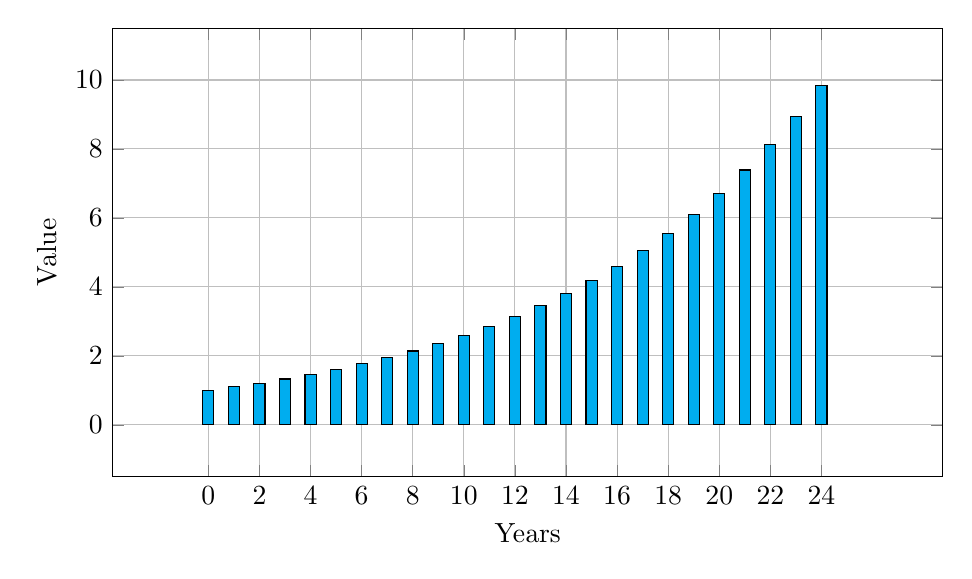
\begin{tikzpicture}
        \begin{axis}[
            width=\textwidth,
            height=0.6\textwidth,
            grid=major,
            xlabel={Years},
            ylabel={Value},
            ymin=0, ymax=10,
            xmin=0, xmax=25,
            ytick={0,2,4,6,8,10},
            xtick={0,2,...,24},
            legend pos=north west,
            bar width=4pt,
            enlargelimits=0.15,
            symbolic x coords={0, 1, 2, 3, 4, 5, 6, 7, 8, 9, 10, 11, 12, 13, 14, 15, 16, 17, 18, 19, 20, 21, 22, 23, 24, 25},
            ymajorgrids=true,
            xmajorgrids=true,
            ]
            \addplot[ybar,fill=cyan] plot coordinates {
                (0,1) (1,1.10) (2,1.21) (3,1.33) (4,1.46) (5,1.61) (6,1.77) (7,1.95) (8,2.14) (9,2.36) (10,2.59)
                (11,2.85) (12,3.14) (13,3.45) (14,3.80) (15,4.18) (16,4.60) (17,5.06) (18,5.56) (19,6.11) (20,6.72)
                (21,7.39) (22,8.13) (23,8.94) (24,9.83)
            };
            % \legend{Value over time}
        \end{axis}
    \end{tikzpicture}
    \caption{Money doubling over time with compound interest.}
    \label{fig:compound_interest}
\end{figure}









\section{Compunding at Various Intervals}
It is traditional to quote the interest rate on a yearly basis but adjust the proportion of that interest rate over each compounding period. Divide a year into $m$ equally-spaced compounding periods.
\begin{itemize}
    \item \textbf{Nominal Interest Rate (annual)}: r
    \item \textbf{Length of a compounding period} : \( \frac{1}{m} \) years
    \item \textbf{Interest Rate for each of the $m$ periods}: : \( r \frac{1}{m} \)
    \item \textbf{Growth of account over $k$ compounding periods}: \((1 + \frac{r}{m})^{k} \)
    \item \textbf{Growth of account over 1 year}: \((1 + \frac{r}{m})^{m} \)
    \item \textbf{The effective interest rate} is the number $r_{\text{eff}}$ such that \((1 + r_{\text{eff}})^{m} = (1 + \frac{r}{m})^{m}\)
\end{itemize}

\section{Continuous Compounding}
Increasing the 